\section{\textbf{Exploring gating/activation mechanisms of TRP channels}}

\section*{Goal and Motivation}
Transient receptor potential (TRP) channels are a large and diverse family of transmembrane ion channels that are critical in sensory perception through polymodal activation by various physical and chemical stimuli.

\begin{figure}[H]
    \centering
    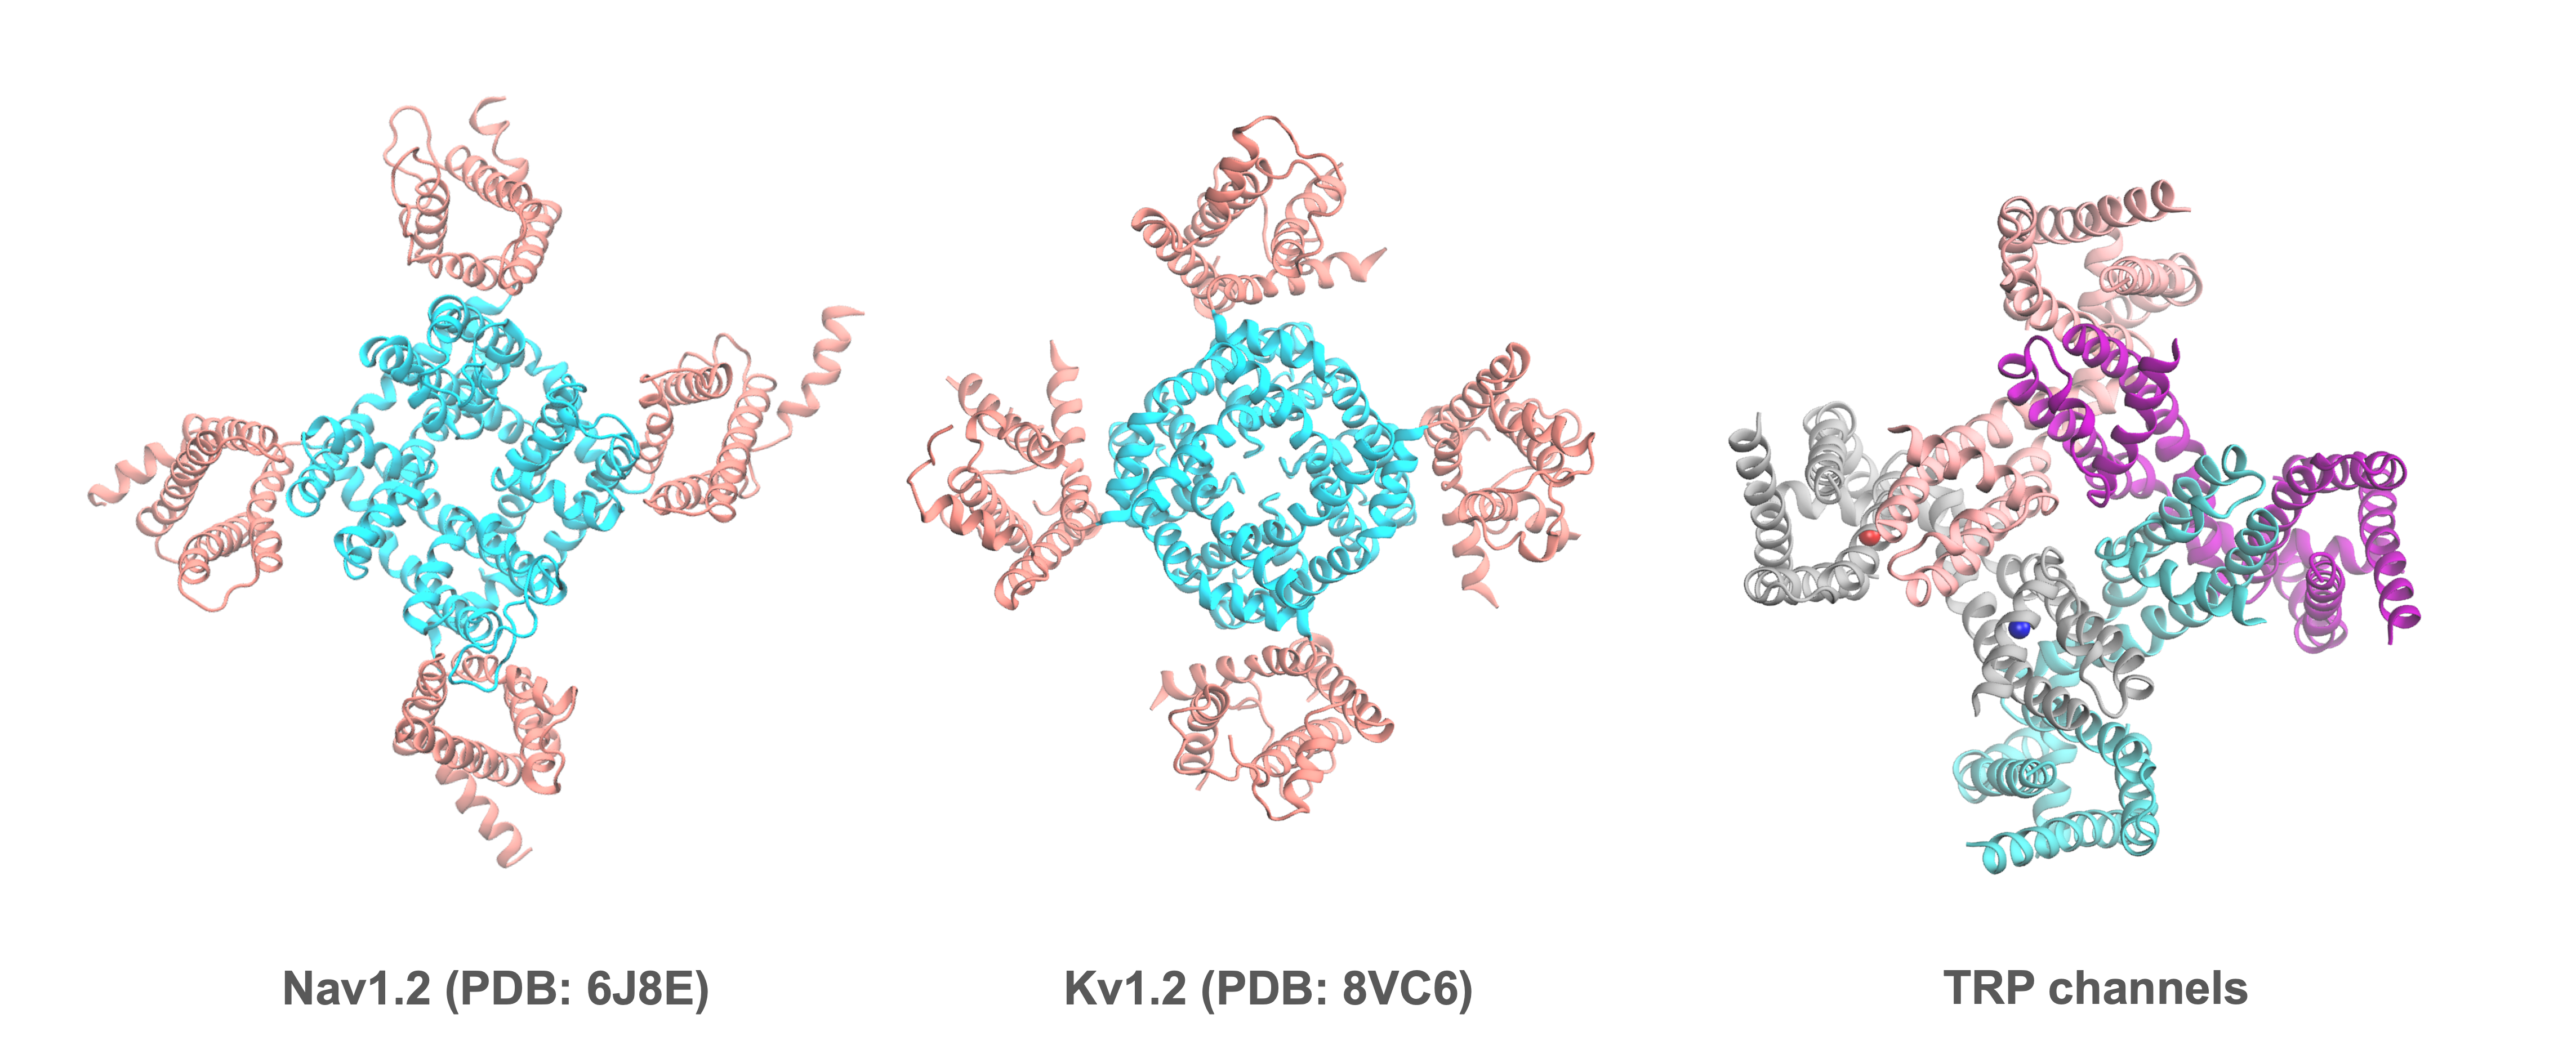
\includegraphics[width=400pt]{topological_similarity.png}
    \caption{The similarity of topologies of voltage-gated ion channels (Nav1.2 and Kv1.2 as two examples shown here) and TRP channels (TRPV4 as an example shown in the right panel). Only the transmembrane region (TM) is shown with the pore region and the voltage sensor domain shown as salmon and cyan color respectively. For TRP channel in the right panel, TMs from four monomers are colored differently in order to show the domain-swapping feature of the topology.}
    \label{fig:topological similarity}
\end{figure}

\newpage